\chapter{Machine learning approach for true track tagging}
Applying cuts to track features in order to differentiate between true and false reconstructed tracks improved their ratio. A more effective
approach in classifying a track as true or false might be achieved with a machine learning algorithm for classification.
Unlike one-dimensional cuts, a machine learning
algorithm can be implemented to benefit from correlations between the input features for a more accurate identification of true tracks. The utilised
machine learning library is XGBoost \cite{xgboost}. It is used for supervised learning problems \cite{supervised} which are explained in the following section.

%\section{Introduction to XGBoost}
\section{Supervised learning}
%XGBoost is a gradient boosting machine learning algorithm \cite{gradient}, which primarily uses decision trees as a predictive model for classification and regression analysis.
Supervised learning is used to predict a target variable $y_i$ based on the training data $x_i$ containing multiple features. The model
in supervised learning describes the mathematical structure, which determines the prediction from its input data.
A linear model is a common example, where the predictions
are linear combinations of the weighted input features:
\begin{align}
  \hat{y}_i = \sum_j \Theta_j x_{ij}
\end{align}
The coefficients $\Theta_j$ are a priori undetermined parameters that need to be learned from the training data.
Therefore, the task of training is in determining the optimal parameters
for the target variable $y_i$ based on the input $x_i$. In order to train a model, an objective function, which measures how well
the model fits the training data, needs to be defined and optimised.
Those functions consist of the training loss function $L(\Theta) $ and the regularization term $\Omega (\Theta)$.
\begin{align}
  \text{obj}(\Theta) = L(\Theta) + \Omega(\Theta)
\end{align}

The training loss function is commonly defined as the mean squared error or logistic loss for logistic regression \cite{logistic}:
\begin{align}
  &L(\Theta) = \sum_i (y_i - \hat{y}_i)^2 \\
  &L(\Theta) = \sum_i [y_i \ln{(1 + \text{e}^{-\hat{y}_i})} + (1 - y_i) \ln{(1 + \text{e}^{-\hat{y}_i})}]
\end{align}
Logistic regression refers to the statistical model that uses logistic functions to model binary dependent variables. \\
The regularization term limits the complexity of a model in order to prevent overfitting. Overfitting occurs when the model fits the training data too well that it adjusts
to random fluctuations with no causal relation. Predictions of new unseen data then become worse, as the learner is not able to generalise well.

\section{Decision tree ensemble}
Decision trees are tree-structured diagrams, which classify a target variable based on a series of decisions. They consist of internal nodes, which denote
a test on an attribute, branches, which represent the outcome of the tests, and leaf nodes, which are the nodes of a decision tree that do not split the data any further. \\
The model used by the XGBoost library is the ensemble of decision trees, which consists of a set of classification and regression trees (CART) \cite{cart}.
A CART assigns a prediction score to each of the leaves.
The prediction of a single tree is usually not sufficiently accurate,
therefore the prediction of numerous trees is summed together. This method can be written mathematically as:
\begin{align}
  \hat{y}_i &= \sum_{k=1}^K f_k(x_i)\,, \: f_k \in \mathcal{F} \\
  \text{obj}(\Theta) &= \sum_i l(y_i, \hat{y}_i) + \sum_{k=1}^K \Omega(f_k)
\end{align}
Where $K$ is the number of trees, $l(y_i, \hat{y}_i)$ is the loss function that measures the difference between the predictions and the
target variable, $\mathcal{F}$ the set of all possible CARTs, and $f$ a decision function of the respective CART. A decision tree ensemble is shown exemplarily in
Figure \ref{fig:random_forest}.

\begin{figure}
  \centering
  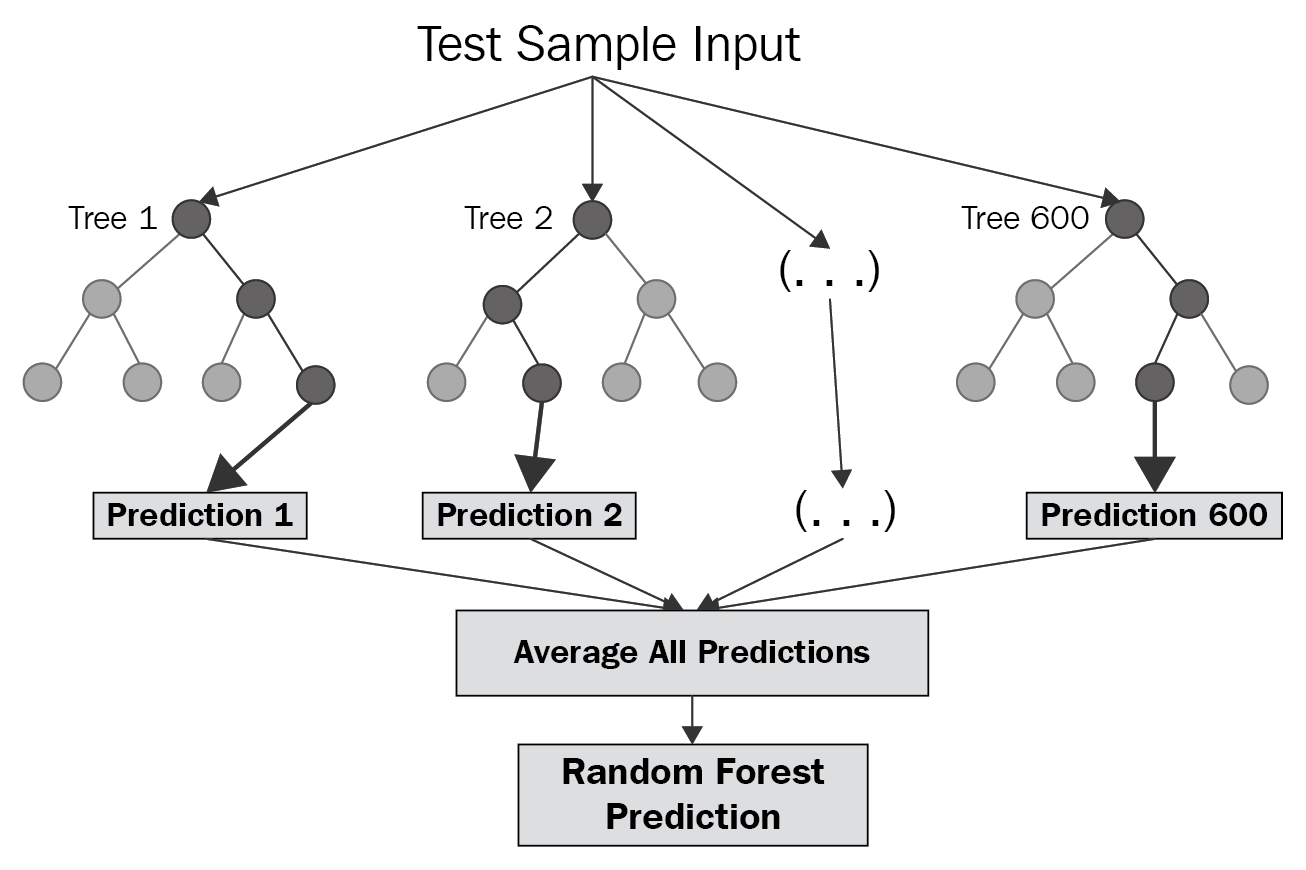
\includegraphics[height=0.6\textwidth]{images/random_forest.png}
  \caption{Representation of a decision tree ensemble \cite{random_forest}.}
  \label{fig:random_forest}
\end{figure}

\section{Boosted trees}
%The model used for boosted trees and a random forest is both the tree ensembles with the only difference being the training method.
%Random forests and boosted decision trees are both tree ensembles that differ only in their training method.
Unlike random forest algorithms \cite{random}, in which a multitude of decision trees are created independently and combined at the end,
it is also possible to build one tree at a time and
combine them iteratively. This method is the gradient boosting machine learning algorithm \cite{gradient}, which is used by XGBoost. \\
Optimising the objective functions for
boosted decision trees (BDT) is achieved by additive training. This means that previous trees are fixed and only one new tree per step $t$ is added.
This can be written
down as follows:
\begin{align}
  \hat{y}_i^{(t)} = \sum_{k=1}^t f_k(x_i) = \hat{y}_i^{(t-1)} + f_t(x_i)
\end{align}

The tree added in each step is supposed to optimise the objective and can be written at step $t$:
\begin{align}
  \text{obj}^{(t)} &= \sum_{i=1} \left[g_i f_t(x_i)] + \frac{1}{2}h_i f_t^2(x_i)\right] + \Omega(f_t)  \\
  g_i &= \partial_{\hat{y}_i^{(t-1)}} l(y_i, \hat{y}_i^{(t-1)}) \\
  h_i &= \partial^2_{\hat{y}_i^{(t-1)}} l(y_i, \hat{y}_i^{(t-1)})
\end{align}
By using the second-order Taylor expansion of the loss function instead of only the first one, a more precise approximation of the loss function is determined in comparison
to regular gradient boosting algorithms \cite{newton_boosting}.
Furthermore, the value of the objective function only depends on $g_i$ and $h_i$, giving XGBoost the advantage of using custom loss functions including logistic regression.
However, the regularisation term still needs to be defined. One definition that works well in practice and is thus used by XGBoost is:
\begin{align}
  \Omega (f) = \gamma T + \frac{1}{2}\lambda \sum_{j=1}^T \omega_j^2
\end{align}
Here, $\omega$ is the vector of scores on leaves, $\gamma$ is the minimum loss reduction required to make
another partition on a leaf, $T$ is the number of leaves, and $\lambda$ is the Ridge regularisation term \cite{ridge}, which shrinks the $\omega_j$ to control the
regularisation term. \\
With this definition, the objective function for a single tree can be compressed to:
\begin{equation} \label{eqn:obj}
  \text{obj} = -\frac{1}{2}\sum_{j=1}^T \frac{G_j^2}{H_j + \lambda} + \gamma T
\end{equation}
Here, $G_j$ and $H_j$ are the sums over all $g_i$ and $h_i$, respectively. Equation \ref{eqn:obj} is a measure of how good a tree structure is. Its structure score
is determined by the statistics $g_i$ and $h_i$ in the leaves, with a smaller score indicating a better tree structure.
Since it is not feasible to enumerate all possible trees to find the best one, only one level at a time is optimised.
For each split of a leaf into a new left leaf L and right leaf R, the gained structure score is defined as:
\begin{equation}
  \text{Gain} = \frac{1}{2}\left[\frac{G_{\text{L}}^2}{H_{\text{L}} + \lambda} + \frac{G_{\text{R}}^2}{H_{\text{R}} + \lambda} - \frac{(G_{\text{L}} + G_{\text{R}})^2}{H_{\text{L}}+H_{\text{R}}+\lambda}\right] -\gamma
\end{equation}

Optimal splits are then determined by calculating the structure score of all possible split solutions. \\

\section{Machine learning setup}
The data used to train the learner %is identical to the one from section \ref{sec:feature} and
consist of 400000 events with ten generated $\SI{200}{\mega\eV}$ protons each
traversing the telescope described in section \ref{sec:setup}. The protons
are reconstructed with Corryvreckan, with the true tracks being identified with the MC truth from Allpix$^2$. A total number of 92546 tracks
are reconstructed, with 36340 being true tracks.
The learner is tested on a previously unseen dataset, simulated with the same configuration used in
\ref{sec:feature} and consists of 100000 protons with ten protons per event.
To determine the optimal number of boosting rounds, early stopping is utilised on a validation set, consisting of 100000 generated protons. This means, that
the model will train until the validation score stops improving for ten consecutive boosting rounds to rule out statistical fluctuations.
The number of boosted rounds is then determined by the highest validation score.
In this case, the validation score refers to the area under the ROC curve, which was explained in \mbox{section \ref{sec:feature}}. \\
The learner performs a logistic regression and outputs a probability for classifying a track as true or false.
A single tree is created in each iteration, called boosting round, to minimise the loss function.

To determine, whether all features are independent of each other, their correlations are calculated, which is shown in Figure \ref{fig:corr}. Here, the correlation
refers to the Pearson correlation coefficient \cite{pearson} describing the ratio of the covariance of two variables and the product of their standard deviations. \\
Most features show only small positive correlations with each other. The most noticeable exceptions are the cluster positions, which correlate particularly high within each
triplet. All charge deposition features and the $\chi^2$ value show almost no correlation with any other features, though this does not necessarily mean that they are
useful features for separating true and false tracks. \\
Less useful features
are not expected to contribute significantly to classification, but also do not disrupt the learning process, as trees do not split as often on variables with little impact.
However, problems may arise by taking too many features into account, as only limited training data is available to compensate for inefficient splits on features.
To prevent too many splits on less useful features,
the cluster positions on the six sensors in the horizontal and vertical direction are not given as input to the machine learner,
due to their high correlation with each other and their overall small number of splits, shown in Figure \ref{fig:importance_global} in the appendix.
Thus, the remaining 15 features include the $\chi^2$, the kink angles, and the charge depositions.
\begin{figure}
  %\centering
  \hspace{-2.5cm}
  \includegraphics[height=1.0\textwidth]{plots/correlation_matrix.pdf}
  \vspace{-1.8cm}
  \caption{The Pearson correlation coefficient of the kink angles, the cluster positions, the charge depositions, and the $\chi^2$ value.}
  \label{fig:corr}
\end{figure}

%All features, including $\chi^2$, kink angles, and charge depositions are selected as input for the classifier. Less useful features
%are not expected to contribute significantly to classification, but also do not disrupt the learning process, as trees do not split as often on variables with little impact.
%Thus, no problems will arise by taking all features into account, as long as the training data is sufficiently large to be able to compensate for inefficient splits on trees.
The parameters, which are predetermined and can not be inferred from the training of the learner, are called hyperparameters. These parameters are used
to control the learning process and need to be tuned to improve the performance of the classifier.
Taking many hyperparameters and hyperparameter values into account comes at the
cost of a large computation time. For this reason, four parameters are chosen to be optimised. These are firstly the maximum depth of each tree, which influences the
complexity of the model and the likeliness of overfitting. With the learning rate $\eta$, overfitting can be alleviated as it shrinks the feature weights
by the specified factor. It takes values from zero to one, with smaller values describing smaller corrections from further trees.
The minimum loss reduction required for an additional partition on a leaf is referred to as $\gamma$. The minimum sum of instance weight $\theta$
needed in a child has a similar impact. Leaf nodes with a sum of weights less than the specified value will prevent further tree partition steps.
Both $\theta$ and $\gamma$ take values from [0, $\infty$[ and are a measure for how complex the model will be.
For these parameters, larger values represent a slower learning algorithm.
%more conservative algorithm, which means that the learner .

A grid search from the python \cite{python} library Scikit-learn \cite{scikit} is used to determine an optimal
value for each of the parameters mentioned above. The values given as input into the grid search
are shown in Table \ref{tab:grid}.

  \begin{table}
    \centering
    \caption{Parameter values of the grid search. The tree depth refers to the maximum depth of a tree, $\eta$ refers to the learning rate,
    $\gamma$ is a threshold for the allowed minimum loss reduction in a partition step, and $\theta$ is the minimum sum of instance weight needed in a child.}
    \begin{tabular}{c c c c}
      \toprule
      tree depth & $\eta$ & $\gamma$ & $\theta$ \\
      \midrule
      3 & 0.05 & 0.5 & 1  \\
      4 & 0.1  & 1   & 25  \\
      5 & 0.3  & 2 & 50  \\
      6 & 0.7  & 5   &  \\
    \end{tabular}
    \label{tab:grid}
  \end{table}
To compare each different combination of the hyperparameter values quantitatively and obtain an estimation of the uncertainty, a 5-fold cross-validation is performed. This means that
the training data set is split into five equally
large sets, with the learner training on four of them and evaluating on the last one. Each of the five sets serves as the test data once, which means that for each
parameter combination five runs are performed. The area under the ROC curve serves as the scoring function to measure how good the prediction on the test data set is.
The mean of the five AUC values represents the score, which is compared in the grid search. Thus, cross-validation helps to compensate for variability in the simulated
data to derive an accurate estimate of the predictive power of the model. \\
The maximal AUC of $0.706(1)$ is achieved with a maximum tree depth of 4, $\eta=0.7$, $\gamma=5$ and $\theta=25$. By setting $\gamma=5$, the result of the grid search of the remaining
parameters can be visualized and is shown in Figure \ref{fig:grid}. \\
Varying the values of the hyperparameters only causes small changes in the mean test AUC, especially the learning rate has a negligible influence on the AUC. Taking the
standard deviations into account shows that the variation of the hyperparameters does not have a significant impact on the performance of the learner.
%makes it impossible to determine whether the best combination of hyperparameters has the highest AUC. However, due to the
%small differences, no significant impact is to be expected in this case.
The above-mentioned hyperparameter values are chosen for training and testing the model, as they belong to  the model with the highest nominal AUC.

\begin{figure}[H]
  \centering
  \includegraphics[height=0.6\textwidth]{plots/grid_search_weights.pdf}
  \caption{The mean test AUC for the different hyperparameter configurations with the error bars indicating the standard deviation of the mean. The
  smaller bars (red, green, pink, yellow) refer to $\eta$, the larger bars (turquoise, orange, purple) to $\theta$ and the point marked in red to the best model.}
  \label{fig:grid}
\end{figure}



\section{Machine learning results}
To compare the performance of the learner on the training and test datasets, the normalised distributions of the output probabilities of tracks being true are investigated.
These are shown in Figure \ref{fig:output} alongside the corresponding differences.

\begin{figure}
  \hspace{-0.45cm}
  %\centering
  \begin{subfigure}{0.51\textwidth}
      \centering
      \includegraphics[height=0.82\textwidth]{plots/output_normed_weights.pdf}
  \end{subfigure}
  \begin{subfigure}{0.51\textwidth}
      %\centering
      \hspace{-0.15cm}
      \includegraphics[height=0.82\textwidth]{plots/output_difference_weights.pdf}
  \end{subfigure}
  \caption{Normalised probability distributions of tracks being true and false for the training and test data set shown on the left.
  The corresponding difference between the performance of the training and test data is shown on the right.}
  \label{fig:output}
\end{figure}

The distributions of the training and test data predictions only show small differences, indicating that no significant overtraining occurs during the training process.
%For both true and false tracks, the greatest deviations are found at their most probable value, between 0.8 and 0.9.
Both true and false tracks have a maximum of around 0.8 as their most probable value, though the peak for the true tracks is higher due to the larger number
of false tracks assigned to small probabilities of being true tracks. While the number of true tracks increases with the assigned probabilities up to
approximately 0.8, the false tracks have a second maximum for small probabilities, which is as high as their maximum around 0.8.
This means that
with the given input, a lot of false combinations of clusters still show similar properties to true tracks.
Also noteworthy is, that a negligible number of tracks has a probability of 0.9 and higher.

The impact of the individual features to classify the reconstructed tracks can be quantified with the number of times each feature was split.
In Figure \ref{fig:importance}, the feature importance scores of the input features are shown. \\
All three features, namely the $\chi^2$ value and the horizontal kink angles  $\phi_{x,3}$ and $\phi_{x,4}$,
proved to be useful for classifying tracks with cuts, have a high feature score, highlighting their importance for separating true and false tracks.
Other features with a high number of splits, like the vertical kink angle of the second sensor,
can still be useful for the learner in combination with other features even though their use for classifying on their own is insignificant.
\begin{figure}
  \centering
  \includegraphics[height=0.6\textwidth]{plots/feature_importance_all.pdf}
  \caption{The number of splits of each feature that is used as input for the learner.}
  \label{fig:importance}
\end{figure}

To evaluate the predictive power of the learner, a ROC curve can be constructed for several thresholds of classifying tracks as true and false based on the
boosted decision tree output.
The ROC curves for the test and training data set are shown in Figure \ref{fig:auc_comparison} alongside
the ROC curves of the feature cuts from section \ref{sec:feature}.
With the AUC of each ROC curve, the performances of the classifying methods can be compared. \\%Table \ref{tab:AUC} lists each of the AUCs.
Only small differences between the ROC curve of the training and test dataset indicate that no significant overfitting occurs.
The ROC curves of the learner have a noticeably higher AUC than the individual feature cuts and have a better ratio of
TPR and FPR for each possible cut, showing the effectiveness
of using machine learning for track classification in comparison to individual feature cuts. For the best combination of cuts, the ratio of the TPR and FPR is still worse than
comparable points on the ROC curve of the test data. This means that for the same FPR of the two methods, the learner consistently achieves a better TPR.

\begin{figure}[H]
  \centering
  \includegraphics[height=0.6\textwidth]{plots/roc_curve_all.pdf}
    \caption{ROC curves of the machine learner for the training and test data set. In comparison, the ROC curves for the individual feature cuts as well as the
    TPR and FPR of the best combination of cuts for all three features are depicted. A black diagonal line, representing random classification, is shown
    in contrast.}
  \label{fig:auc_comparison}
\end{figure}

%\begin{table}
%  \centering
%  \begin{tabular}{c | c c c c c}
%    \toprule
%      & Train & Test & $\chi^2$ & $\phi_{x,3}$ & $\phi_{x,4}$\\
%    \midrule
%    AUC & 0.770 & 0.754 & 0.615 & 0.617 & 0.587 \\
%  \end{tabular}
%  \caption{Area Under the Curve for the feature cuts and the train and test data of the machine learner.}
%  \label{tab:AUC}
%\end{table}
Further optimisation of the machine learning results is possible, considering that each cluster can at most be associated with one true track.
Only keeping the track of clusters with the highest probability of being true enables further rejection of
false tracks. The ROC curve of the test data with the rejection of tracks is shown in Figure \ref{fig:rejection}. \\
With the rejection of tracks, the AUC on the test data set decreases to $0.702$. This is due to the rejection of many true negative tracks, which in turn increases
the false positive rate. Since the goal is to improve the quality of the pCT image, the false positive rate is not an ideal quantity, as true negative tracks
are not taken into account for pCT anyway.
%However, the rejection of true negative tracks does not decrease the quality of the pct image, as these tracks are not taken into account anyway.

\begin{figure}[H]
  \centering
  \includegraphics[height=0.6\textwidth]{plots/roc_curve_learner_rejection_weights.pdf}
  \caption{ROC curves of the training and test data set and the test data set including the rejection of all but one track from clusters on the first and last plane.}
  \label{fig:rejection}
\end{figure}

To evaluate this method, the precision score $P=t_p/(t_p + f_p)$ and the recall score $R=t_p/(t_p + f_n)$ are calculated and compared with the baseline classifier. The precision
score describes the ability of the learner to not classify negative events as positive. The recall score, referring to the same quantity as the true positive rate,
is the ability to classify all positive events correctly.
Figure \ref{fig:precision} shows the precision of the learner and the individual feature cuts as a function of the recall.

%\begin{figure}
%  \hspace{-0.6cm}
%  %\centering
%  \begin{subfigure}{0.51\textwidth}
%      \centering
%      \includegraphics[height=0.82\textwidth]{plots/roc_curve_precision_train.pdf}
%  \end{subfigure}
%  \begin{subfigure}{0.51\textwidth}
%      %\centering
%      %\hspace{0.95cm}
%      \includegraphics[height=0.82\textwidth]{plots/feature_cuts_precision.pdf}
%  \end{subfigure}
%  \caption{Precision as a function of the recall for the train and test data set including the rejection of all but one track from clusters of the first and last
%           sensor for the test dataset. As a comparison, the precision curves are also shown for cuts on the $\chi^2$, $\phi_{x,3}$, and $\phi_{x,4}$ features.}
%  \label{fig:precision}
%\end{figure}

\begin{figure}[H]
  \centering
  \includegraphics[height=0.6\textwidth]{plots/roc_curve_precision_all.pdf}
  \caption{Precision as a function of the recall for the training and test data set including the rejection of all but one track from clusters of the first and last
           sensor for the test dataset. As a comparison, the precision curves are also shown for cuts on the $\chi^2$, $\phi_{x,3}$, and $\phi_{x,4}$ features.}
  \label{fig:precision}
\end{figure}
The AUC of the precision curve increases with the rejection of tracks,
indicating a better performance with the rejection method. In comparison to the regular test data set, the precision score
of the test data set with the rejection of tracks increases noticeably for recall scores larger than 0.1.
%This is also reflected in the AUC values of the curves, with the precision curve of the rejection method having the highest AUC.
Furthermore, a higher precision score of the test data set in comparison to the individual feature cuts for all recall scores highlights the advantages of the machine
learning approach. The precision is especially stable for the test dataset with the rejection method for recall scores larger than $0.1$,
which means that high recall scores
are achievable without decreasing the precision score significantly.
However, this also means that no working point can be chosen that has an exceptionally high precision score. Useful choices for working points might be around
a recall score of $0.8$ with a precision score of approximately $0.636$ due to a noticeable decrease of precision for higher recall scores.
